\chapter{Projekt i~implementacja systemu}

Autor nazwał system HelloReview (HR). Informacja ta ma charakter porządkowy, nazwa ta, lub jej skrót, występuje na załączonych rysunkach, może także wystąpić w~tekście.

Przepływ danych w~systemie wygląda następująco:

\begin{enumerate}
    \item Użytkownik loguje się do systemu następuje przy użyciu konta GitHub;
    \item Prowadzący zakłada kursy, do których zapisuje kursantów;
    \item Prowadzący tworzy projekt z~zadaniem na platformie GitHub;
    \item Kursant rozwiązując zadanie powielają odpowiedni projekt na platformie GitHub;
    \item Prowadzący zleca wzajemną ocenę postępów pracy dla danego projektu;
    \item Kursant ocenia pracę innego studenta wypełniając ankietę;
    \item Prowadzący sprawdza odpowiedzi w~systemie.
\end{enumerate}

Taki przebieg wydarzeń uwzględnia wszystkie wymagania w~stosunku do projektowanego systemu. W~rozdziale tym przedstawione zostaną szczegóły projektowe i~implementacyjne na bazie przedstawionych punktów. Przedstawienie projektu za zasadzie chronologicznie ułożonych wydarzeń ma na celu ułatwienie odbioru pracy, oraz zrozumienia budowy i~zasady działania systemu.

\newpage
\section{Logowanie do systemu}
Niezalogowany użytkownik po uruchomieniu strony internetowej nie posiada żadnych uprawnień. Zastaje on widok jak na zrzucie ekranowym na rysunku \ref{obr11}. Jedyną przewidzianą akcją w~tym momencie jest logowanie do systemu.

\begin{figure}[!h]
\centering
    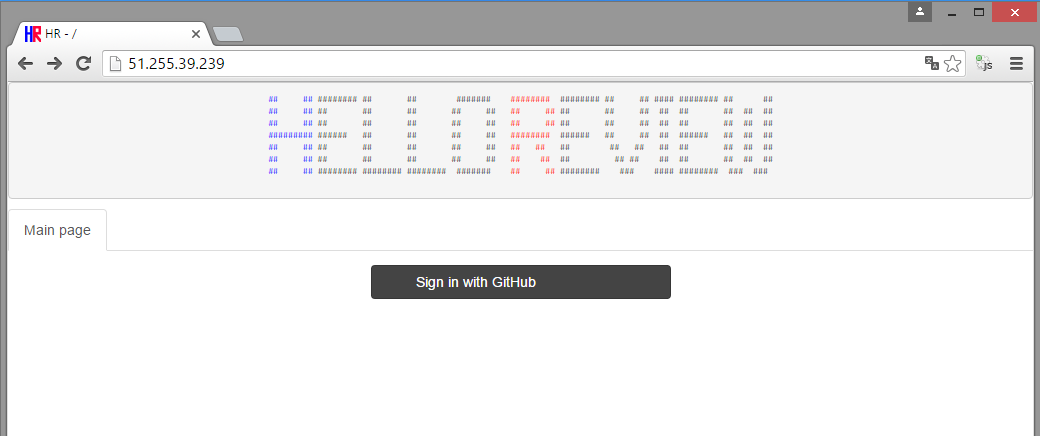
\includegraphics[width=\textwidth]{1_1logowanie}
    \caption{Zrzut ekranowy: strona główna dla niezalogowanego użytkownika}
    \label{obr11}
\end{figure}

Logowanie do systemu odbywa się przy użyciu usługi GitHub jako serwera autoryzacji. Autoryzacja następuje przy użyciu protokołu OAuth2. Użytkownik po kliknięciu w~przycisk zostaje przekierowany do platformy GitHub, gdzie potwierdza chęć udostępnienia danych systemowi, który go skierował. Wygląd potwierdzenia autoryzacji dla aplikacji przedstawia zrzut ekranowy na rysunku \ref{obr12}.

\begin{figure}[!h]
\centering
    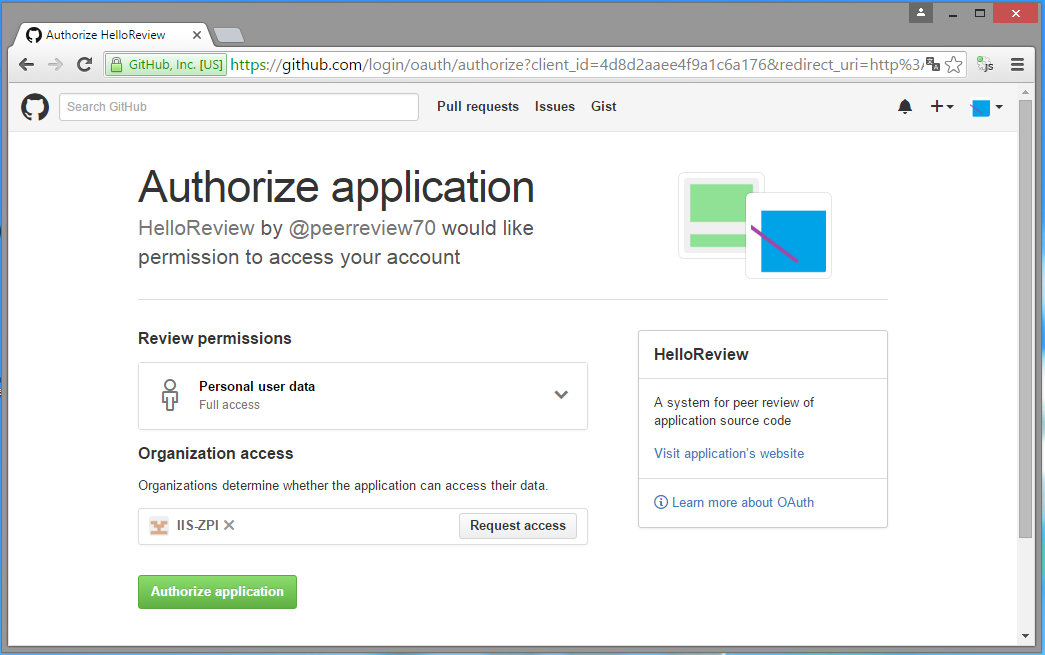
\includegraphics[width=375px]{1_2github}
    \caption{Zrzut ekranowy: autoryzacja aplikacji w~serwisie GitHub}
    \label{obr12}
\end{figure}

Jeżeli użytkownik potwierdził autoryzację system otrzymuje token autoryzacyjny, za pomocą którego może odczytać podstawowe dane na temat użytkownika. Najważniejszą informacją udostępnianą przez serwis GitHub jest nazwa użytkownika. To na jej podstawie system określa uprawnienia. Jeżeli nazwa zalogowanego użytkownika znajduje się w~pliku konfiguracyjnym, na liście w~sekcji \textquote{masters} to uzyskuje on dostęp z~prawami prowadzącego. W~przeciwnym razie ma on uprawnienia kursanta. Użytkownik, który nie zgodził się na udostępnienie danych nie może korzystać z~systemu. Wyrażenie braku zgody polega na zamknięciu zakładki z~akcją potwierdzenia, a~więc przerwaniu procesu potwierdzenia i~opuszczeniu systemu.

\medskip
Charakter systemu powoduje, że nie ma tu stopniowania uprawnień. Uprawnienia są rozłączone, co ułatwiło implementację kontroli uprawnień. Wszystkie podstrony pasujące do wzorca \textquote{/m/**} są przeznaczone dla prowadzącego, wzorzec \textquote{/p/**} odpowiada podstronom dedykowanym kursantom. Inne zasoby są ogólnodostępne, ich zawartość może być pobrana przez każdego - są to pliki statyczne, strona główna, oraz strony błędów.

\medskip
Kontrola uprawnień została zaimplementowana wykorzystując mechanizm \textquote{przechwytywania} (ang. intercept) żądań. Przed przejściem do właściwego kontrolera Spring uruchamia zdefiniowane mechanizmy wykonujące autoryzację. Rysunek numer \ref{kodi1} na stronie \pageref{kodi1} zawiera listing kodu z~klasą \textquote{InterceptorRegistryConfig}. Odpowiada ona za zarejestrowanie klas typu \textquote{interceptor}. Dwie z~zarejestrowanych klas są odpowiedzialne za kontrolę uprawnień. \textquote{InterceptorHasRoleMaster} sprawdza uprawnienia do podstron dla prowadzącego, oraz odpowiednio \textquote{InterceptorHasRoleMaster} sprawdza uprawnienia dla podstron dla kursantów.

\medskip
Rysunek numer \ref{kodi2} na stronie \pageref{kodi2} zawiera listing kodu z~klasą \textquote{InterceptorHasRoleMaster}. Autoryzacja polega na odpytaniu biblioteki pac4j, czy aktualnie użytkownik jest zalogowany, oraz sprawdzenie, czy jego nazwa użytkownika widnieje w~konfiguracji jako poprawna nazwa konta prowadzącego. Do komunikacji z~biblioteką pac4j autor napisał dodatkowo klasę użytkową \textquote{GHPac4jSecurityHelper}, która eksponuje jedynie rzeczy istotne dla systemu. Jeżeli użytkownik jest niezalogowany zostaje przekierowany do strony głównej. W~przypadku wykrycia próby uzyskania dostępu do zasobów przez zalogowanego użytkownika, do których nie ma uprawnień wysyłana jest odpowiedź ze stroną błędu o~kodzie \textquote{401 Unauthorized}. Autoryzacja uprawnień do podstron dla kursanta wygląda w~sposób odpowiadający - za kursanta system uważa każdego, kto nie został rozpoznany jako prowadzący.

\begin{figure}[!h]
\centering
    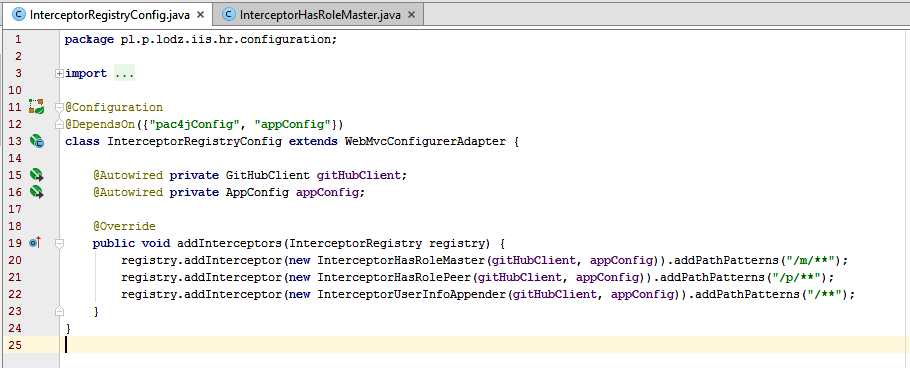
\includegraphics[width=\textwidth]{kod_interceptor1}
    \caption{Listing kodu źródłowego: klasa InterceptorRegistryConfig}
    \label{kodi1}
\end{figure}

\begin{figure}[!h]
\centering
    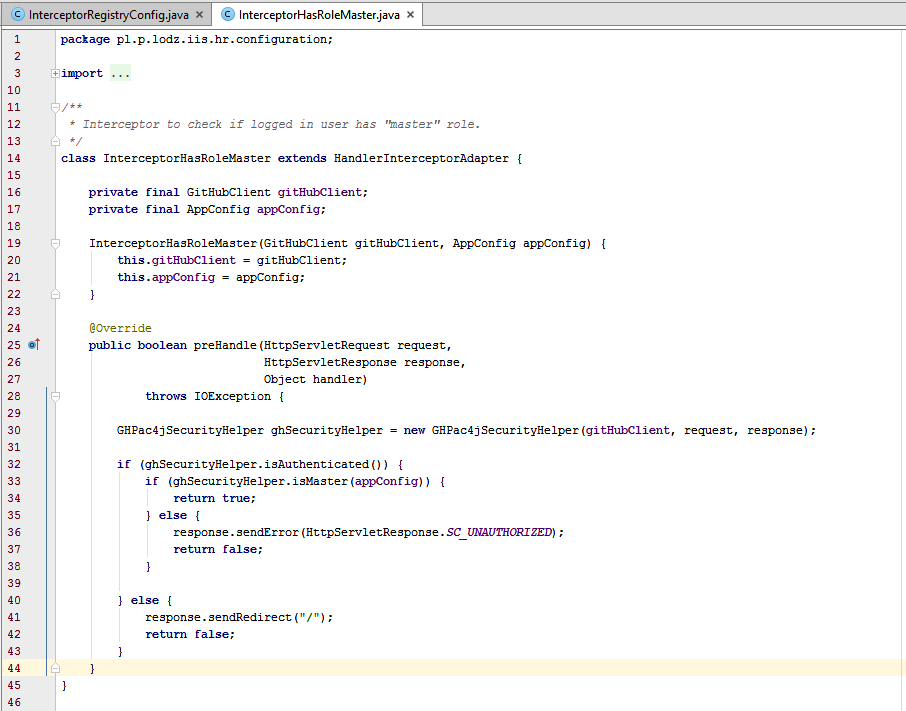
\includegraphics[width=\textwidth]{kod_interceptor2}
    \caption{Listing kodu źródłowego: klasa InterceptorHasRoleMaster}
    \label{kodi2}
\end{figure}

\clearpage
\section{Kursy i~ich uczestnicy}
Korzystanie z~systemu należy rozpocząć od zarejestrowania kursu i~przypisania do nich uczestników. System został tak zorganizowany, że na każdej podstronie widnieje lista znajdujących się zasobów danego typu (w~postaci tabelarycznej), a~pod nią przycisk dodania kolejnego. Obrazki \ref{obr21}, \ref{obr22}, \ref{obr23} zawierają kolejno zrzuty ekranowe przedstawiające: przykładową listę kursów, przykładową listę kursantów, i~przykład próby dodania kursu zakończonego niepowodzeniem, z~powodu niepowodzenia walidacji wprowadzonych danych.

\medskip
Kurs identyfikuje jedynie jego nazwa (ang. course name). W~przypadku kursanta należy podać dwie wartości: personalia (zwykle imię i~nazwisko) (ang. participant name) i~nazwę konta w~systemie GitHub (ang. GitHub nick, GitHub name). Poszukiwanie informacji dla danego kursanta, gdy ten się zaloguje do systemu, polega na porównaniu nazwy konta, z~którego się zalogował z~istniejącymi wpisami na temat uczestników w~bazie danych. Jest to jedyny warunek kontroli uprawnień do zasobów kursanta. Tożsamość została już wcześniej potwierdzona i~powiązana z~nazwą konta. Na tym etapie jest to warunek konieczny i~zupełnie wystarczający.

\medskip
\begin{figure}[!h]
\centering
    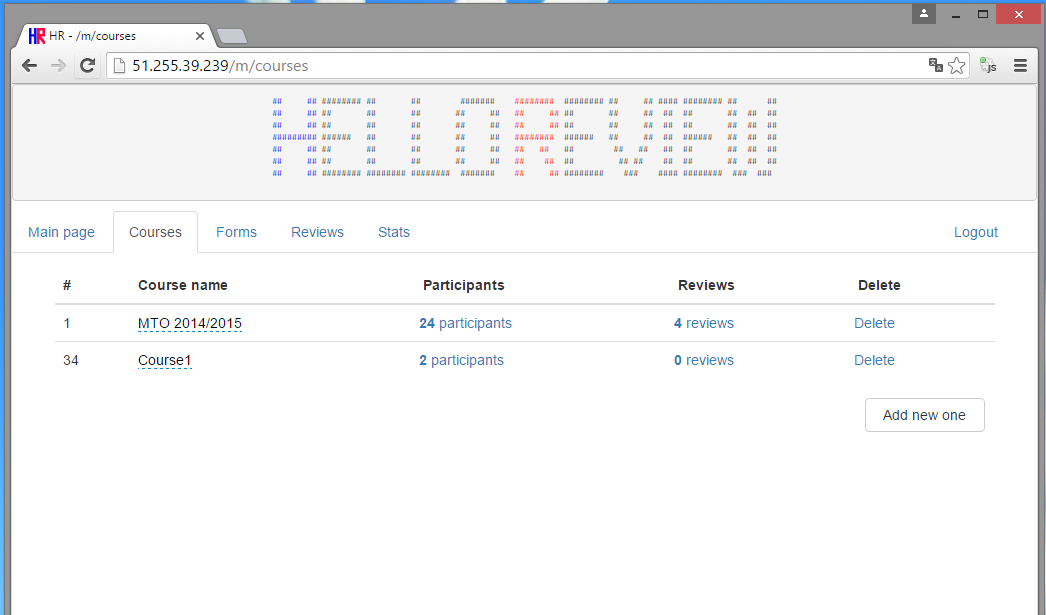
\includegraphics[width=\textwidth]{2_1kursy}
    \caption{Zrzut ekranowy: lista kursów}
    \label{obr21}
\end{figure}

\begin{figure}[!h]
\centering
    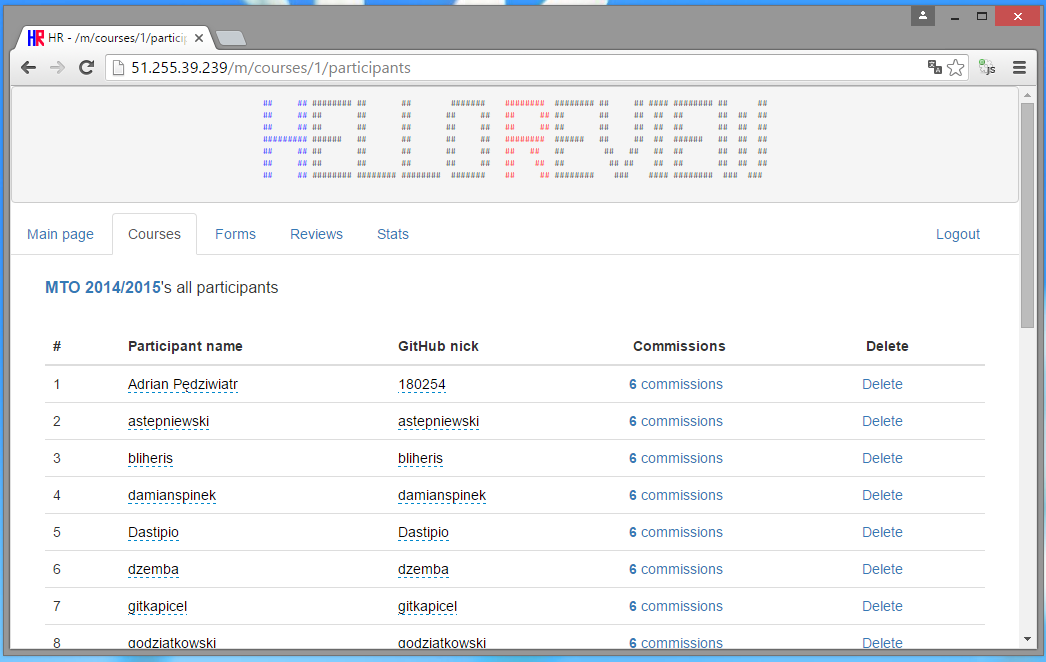
\includegraphics[width=\textwidth]{2_2kursanci}
    \caption{Zrzut ekranowy: lista kursantów}
    \label{obr22}
\end{figure}

\begin{figure}[!h]
\centering
    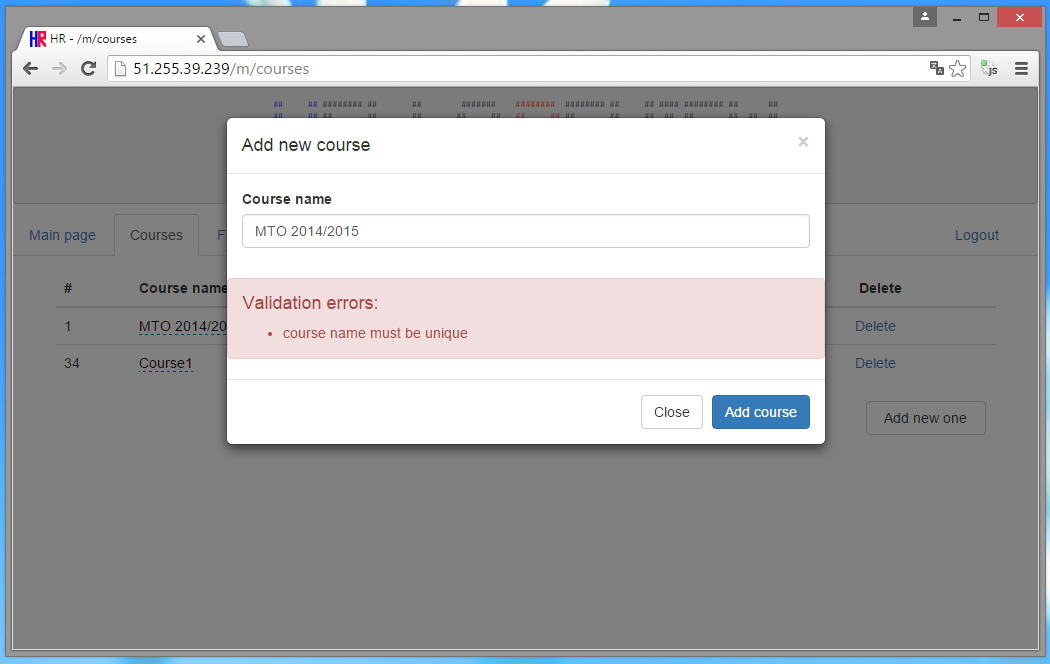
\includegraphics[width=\textwidth]{2_3dodanie}
    \caption{Zrzut ekranowy: formularz dodania kursu}
    \label{obr23}
\end{figure}

\clearpage
\section{Prowadzący umieszcza zadanie na platformie GitHub}
Prowadzący umieszcza dla każdego zadania nowe repozytorium Git na platformie GitHub. Przy czym nie chodzi tutaj o~umieszczenie w~nim samej treści zadania, a~o~projekt zawierający kod startowy. Założenie było wzorowane na laboratoriach, gdzie taki projekt bazowy zawierał kod, który należało rozbudować, poprawić lub uzupełnić o~przypadki testowe. Nic nie stoi na przeszkodzie jednak, by repozytorium takie było podstawowym ogólnym szablonem i/lub zawierało treść polecenia. Istotne jest jednak, że dla każdego zadania należy utworzyć oddzielne repozytorium.

\medskip
Założeniem jest jedno repozytorium = jeden przegląd, jedna ocena. Zgrupowanie zadań powoduje więc jednocześnie, że możliwość zlecenia przeglądu także istnieć będzie jedynie grupowo. Istnieje możliwość sprostowania, np. poprzez napisanie komentarza do zlecenia przeglądu, lecz użytkownik dostanie kopię całego repozytorium. Próba grupowania wydaje się więc być zbędną kombinacją, mimo wszystko możliwą jednak do realizacji.

\medskip
Dla systemu nie są istotne nazwy repozytoriów. Przykładową konwencją może być np. \textquote{lab\textunderscore X-Y}, gdzie X to kolejny numer zajęć, natomiast Y to numer zadania w~ramach danych zajęć.

\clearpage
\section{Kursant powiela repozytorium z~zadaniem}
Kursant rozwiązanie zadania rozpoczyna od powielenia (ang. fork) repozytorium na platformie GitHub. W~ten sposób system rozpoznaje, że kursant rozpoczął proces wykonania zadania, i~znajduje jego rozwiązanie. Z~uwagi na specyfikę dostępu do zasobów przy użyciu GitHub API istotne jest, aby kursant powielił projekt źródłowy. Błędem jest wielokrotne powielenie. Wielokrotne powielenie należy rozumieć jako powielenie repozytorium z~konta \textquote{X}, które jest powieleniem ze źródłowego konta \textquote{Y}. Należy mieć na uwadze opisane ograniczenie i~poinformować o~nim kursantów. Nieprawidłowe powielenie skutkować będzie nie wykryciem rozwiązania kursanta przez system, co może budzić różne konsekwencje, w~zależności od woli prowadzącego kurs. Rysunek numer \ref{obr41} zawiera zrzut ekranowy z~platformy GitHub, na którym widać, iż projekt został wielokrotnie powielony, lecz kursant o~nazwie konta \textquote{grzego699} wykonał to nieprawidłowo (w~rozumieniu ograniczeń systemu).

\begin{figure}[!h]
\centering
    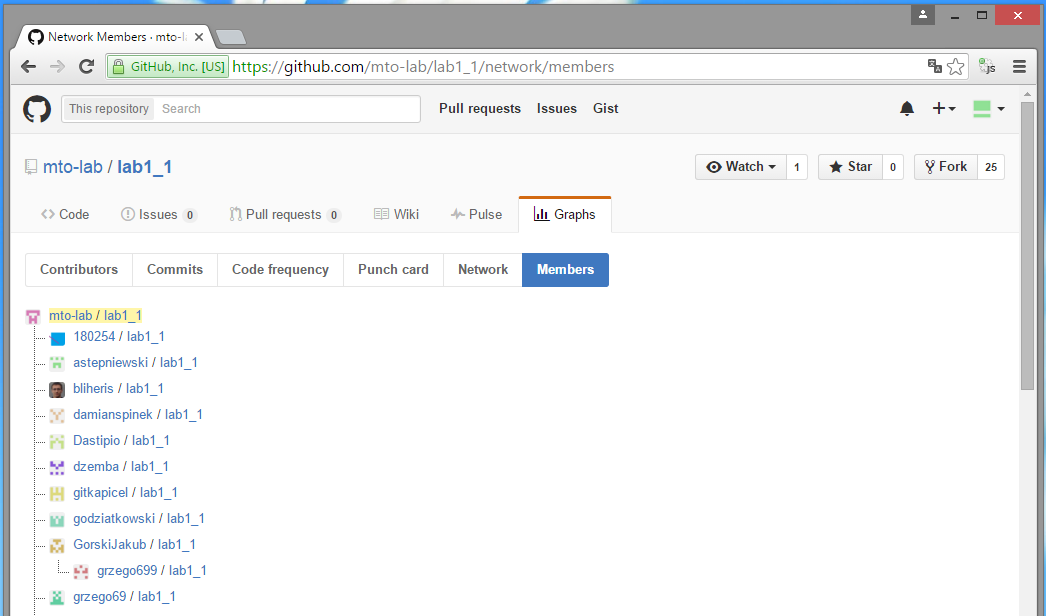
\includegraphics[width=\textwidth]{4_1forks}
    \caption{Zrzut ekranowy: powielenia repozytorium na platformie GitHub}
    \label{obr41}
\end{figure}

\clearpage
\section{Prowadzący zleca przegląd}

\subsection{Formularz oceny}
Jedną ze składowych przeglądu jest formularz, za pomocą którego będzie dokonana ocena. Przed przejściem do właściwej części zlecenia przeglądu należy zastanowić się, czy zastosowanie ma jakiś z~istniejących już w~systemie formularzy, czy też należy dodać następny. 

\medskip
W skład formularza wchodzą następujące składowe:
\begin{itemize}
    \item opis (ang. description) - ogólny informacja dla studenta na temat zadania, które ma aktualnie wykonać (przegląd i~ocena). Opis powinien zawierać dwa znaczniki specjalne \{project\} i~\{url\}. Pierwszy z~nich zostanie w~ostatecznej wersji zastąpiony nazwą projektu (tj. repozytorium), którego ocena następuje. Drugi natomiast zostanie zamieniony na adres do anonimowej kopii, gdzie kursant może się zapoznać z~ocenianą pracą;
    \item pytania (ang. questions) - lista pytań, na które kursant musi odpowiedzieć.
\end{itemize}

\medskip
Pytanie w~formularzu składa się z~następujących składowych:
\begin{itemize}
    \item tekst pytania (ang. question text) - treść pytania;
    \item dodatkowe wskazówki (ang. additional tips) - dodatkowa treść umieszczana zaraz pod treścią główną pytania. Jej przeznaczeniem jest przekazanie kursantowi dodatkowych wskazówek (np. na co powinien zwrócić szczególną uwagę), czy też dowolna inna treść uzupełniająca pytanie. Element ten nie jest obowiązkowy i~nie musi być w~pytaniu wykorzystywany;
    \item kontrolki (ang. inputs) - pola, które służą do wprowadzenia odpowiedzi na pytanie przed kursanta. System obecnie obsługuje dwa rodzaje kontrolek. Kontrolka typu tekst (ang. text) pozwala na wprowadzenie dowolnej treści tekstowej do 10 000 znaków. Kontrolka typu skala (ang. scale) pozwala wyrazić ocenę w~skali liczbowej. Zakres skali, oraz jej znaczenie semantyczne jest bez znaczenia w~sensie technicznym. Pytanie może składać się z~wielu kontrolek - brak jest ograniczeń w~tym względzie. Podczas generowania formularza ich kolejność zostanie zachowana. Kontrolka może zostać oznaczona jako obowiązkowa do wypełnienia lub nie. Z~powodu ograniczeń technicznych systemu parametr ten ma zastosowanie tylko dla kontrolki typu tekst. Wypełnienie kontrolki typu skala zawsze jest obowiązkowe.
\end{itemize}

\clearpage
\medskip
Formularz do systemu wprowadza się poprzez plik XML o~odpowiedniej strukturze. Struktura ta jest sprawdzana pod kątem obecności wszystkich obowiązkowych składowych i~poprawności składniowej. System pozwala na wyświetlenie struktury XML już zdefiniowanych formularzy. Możliwy jest także podgląd wyglądu formularza po jego wygenerowaniu. Wyświetlony formularz jest identyczny z~tym, który zostanie wyświetlony kursantowi. Rysunki o~numerach \ref{obr511}-\ref{obr513} zawierają zrzuty ekranowe z~procesu dodawania formularza do systemu.

\medskip
Plik XML podany przez użytkownika jest przetwarzany na klasę \textquote{Form}, będąca jednocześnie encją. Za tą formę \textquote{deserializacji} odpowiada biblioteka \textquote{Jackson}. Następnie system sprawdza, czy przekazany formularz jest prawidłowy. Kontrola ta polega na upewnieniu się, że wszystkie wymagane pola zostały uzupełnione i~nie są puste. Za proces walidacji odpowiada zastosowana biblioteka \textquote{Hibernate}, a~dokładnie moduł który nazywa się \textquote{Hibernate Validator}. W~przypadku niepowodzenia walidacji prowadzący otrzymuje odpowiednie szczegóły, niezbędne do jego poprawienia. Jeżeli kod formularza okazał się być prawidłowy encja zostaje zapisana w~bazie danych i~podgląd formularza może zostać wyświetlony użytkownikowi.

\begin{figure}[!h]
\centering
    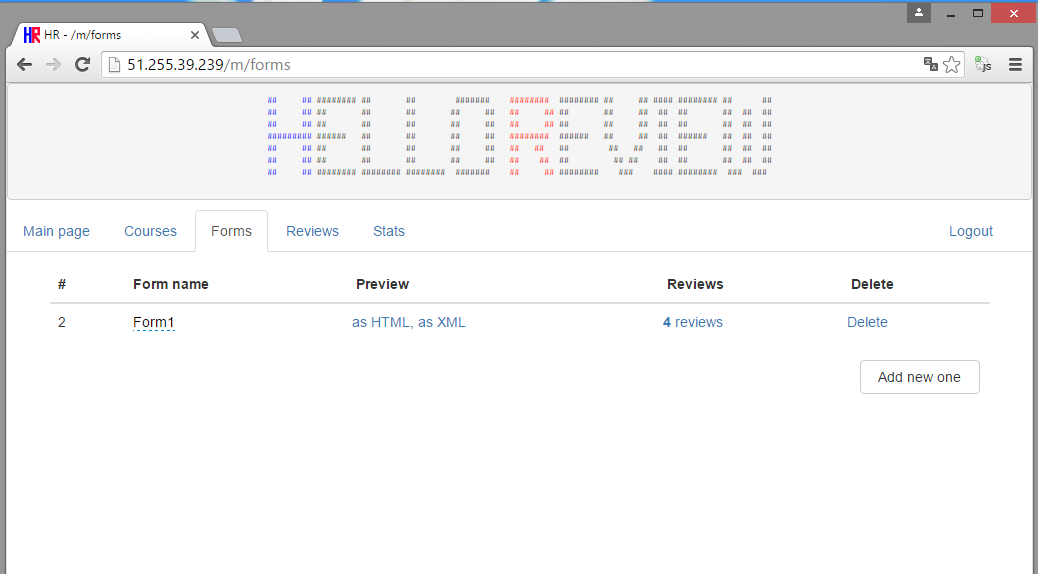
\includegraphics[width=\textwidth]{5_1_1formlist}
    \caption{Zrzut ekranowy: lista formularzy w~systemie}
    \label{obr511}
\end{figure}


\begin{figure}[!h]
\centering
    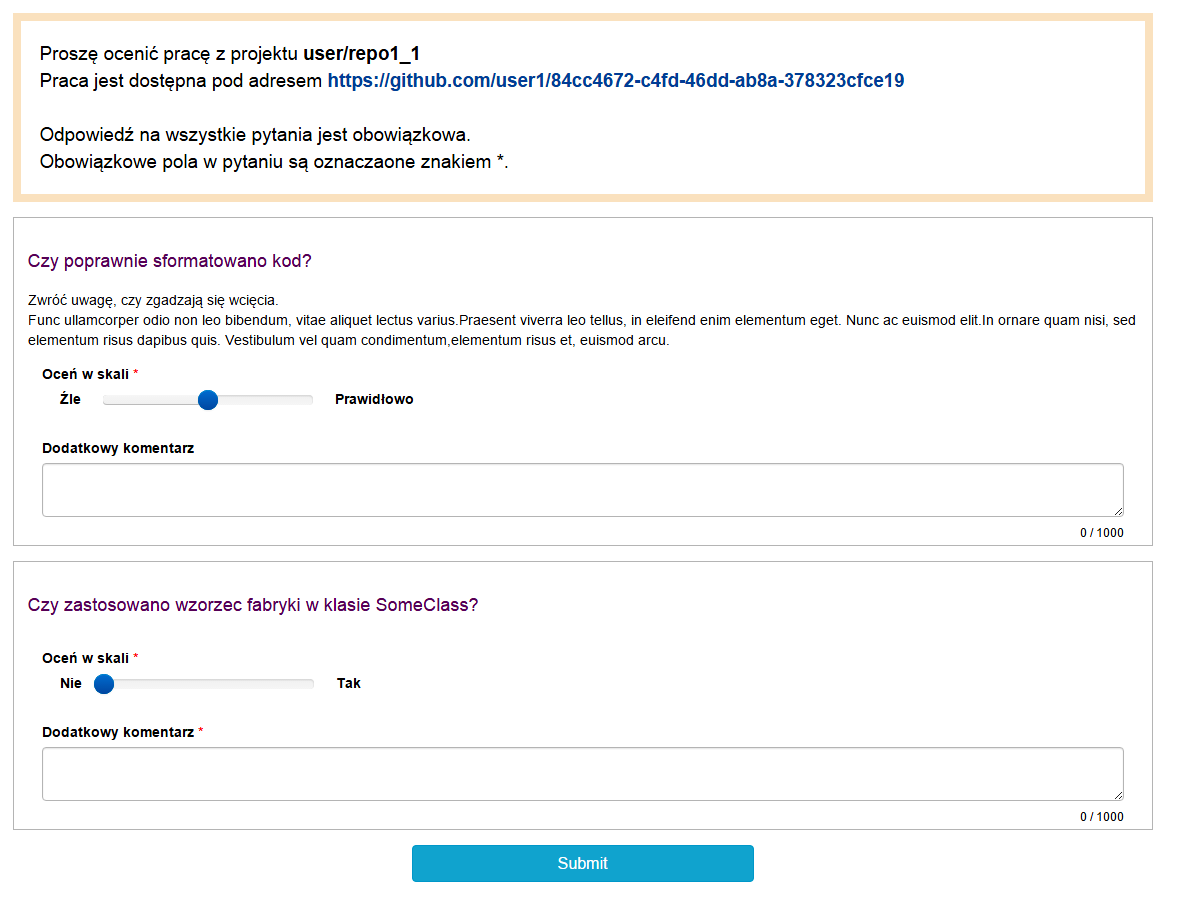
\includegraphics[width=\textwidth]{5_1_2poglad}
    \caption{Zrzut ekranowy: podgląd formularza po jego wygenerowaniu}
    \label{obr512}
\end{figure}


\begin{figure}[!h]
\centering
    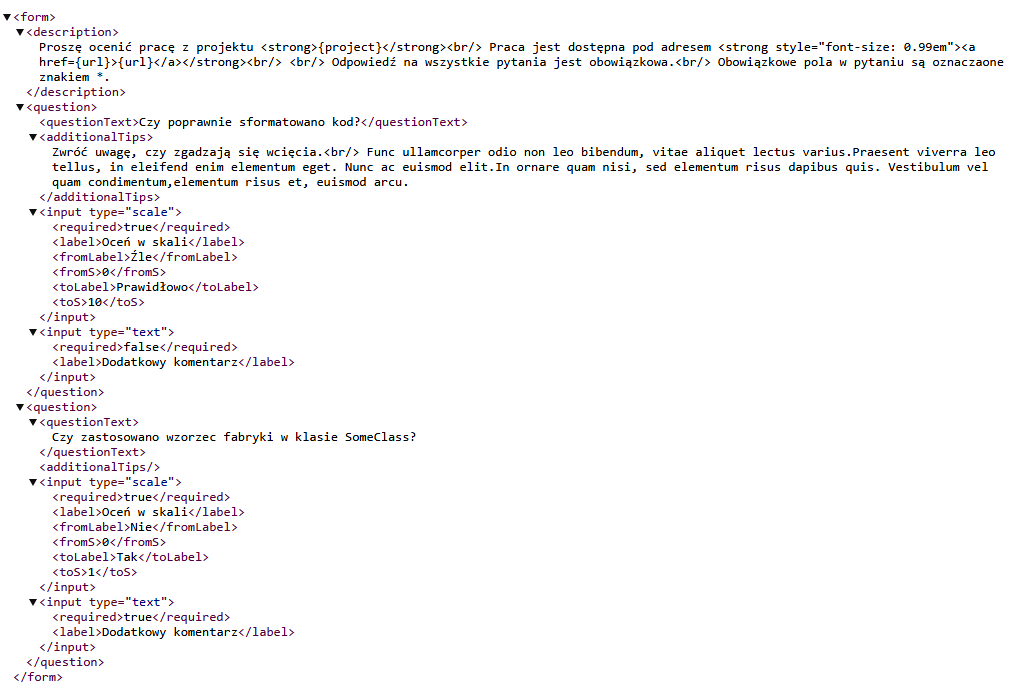
\includegraphics[width=\textwidth]{5_1_3xml}
    \caption{Zrzut ekranowy: przykładowy plik XML z~definicją formularza}
    \label{obr513}
\end{figure}

\clearpage
\subsection{Zlecenie przeglądu}
Rysunek numer \ref{obr521} zawiera zrzut ekranowy z~listą przeglądów w~systemie. Lista jest przedstawiona w~sposób tabelaryczny i~zawiera następujące informacje:
\begin{itemize}
    \item nazwa przeglądu (ang. review name);
    \item odnośnik do kursu (ang. course) związanego z~przeglądem;
    \item odnośnik do formularza (ang. form) związanego z~przeglądem;
    \item odnośnik ocenianego projektu (repozytorium; ang. repository) związanego z~przeglądem;
    \item liczba zleceń oceny na osobę (ang. commissions per peer);
    \item odnośnik do statusu zleceń (ang. commissions);
    \item odnośnik do odpowiedzi (ang. responses);
    \item status zamknięcia (ang. close state).
\end{itemize}

\begin{figure}[!h]
    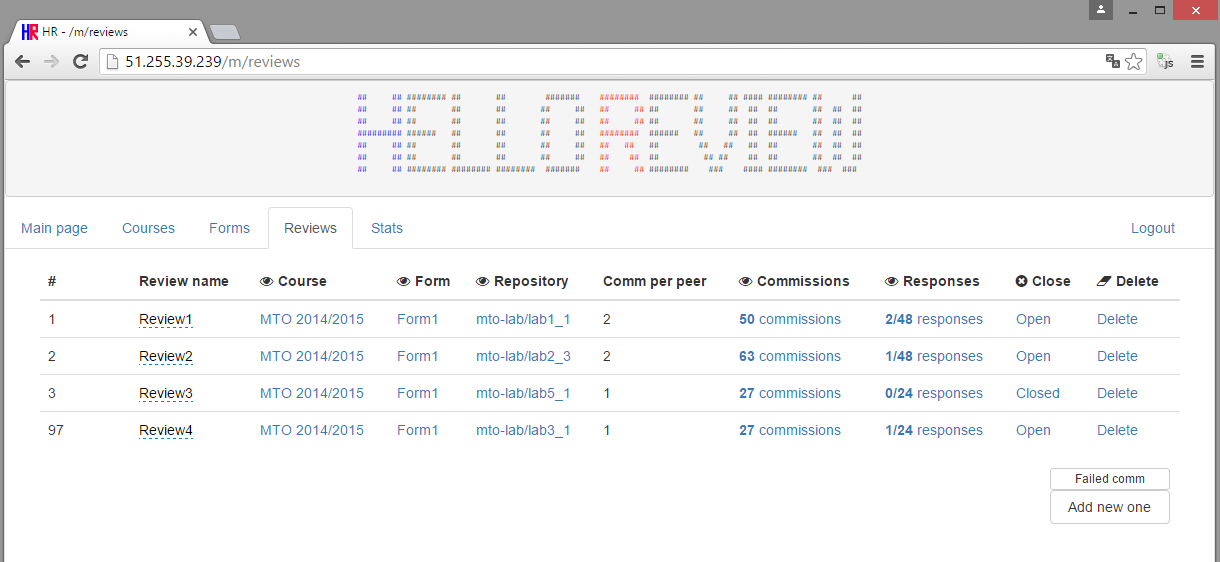
\includegraphics[width=\textwidth]{5_2_1rlista}
    \caption{Zrzut ekranowy: lista przeglądów w~systemie}
    \label{obr521}
\end{figure}

\medskip
Pod listą stworzonych już przeglądów, zgodnie z~zastosowaną konwencją, znajduje się przycisk do formularza, za pomocą którego możliwe jest dodanie nowego przeglądu. Wygląd formularza przedstawia zrzut ekranowy na rysunku \ref{obr523}.

\medskip
Formularz dodawania przeglądu wymaga podania następujących informacji:
\begin{itemize}
    \item nazwa przeglądu (ang. review name) - unikatowa nazwa nowo tworzonego przeglądu;
    \item liczba zleceń na kursanta (ang. number of commissions per participant) - określa ile prac ma ocenić każdy z~kursantów. Przydział prac do oceniania jest losowy. Nie ma jednak możliwości, by kursant dostał dwa tą samą pracę do ocenienia. Nie ma też możliwości ręcznego dokonania przydziału; 
    \item kurs związany z~przeglądem (ang. course) - należy wskazać z~listy kurs, dla którego zostanie utworzony przegląd;
    \item formularz związany z~przeglądem (ang. form) - należy wskazać z~listy formularz, który zostanie użyty do oceny;
    \item repozytorium projektu związanego z~przeglądem (ang. repository) - należy wskazać repozytorium projektu, którego rozwiązania kursanci mają dokonać oceny. 
\end{itemize}

\medskip
Przegląd jest pojęciem ogólnym i~dotyczy zadania w~ramach grupy - prowadzący zlecił dokonanie przeglądu danego zadania, w~danej grupie. Przegląd składa się ze zleceń. Zlecenie jest to pojedyncze zadanie ocenienia pracy autorstwa~A przez osobę~B.

\medskip
Po potwierdzeniu chęci wykonania przeglądu poprzez przycisk \textquote{stwórz przegląd} (ang. create review) system dokona sprawdzenia, czy wszyscy kursanci prawidłowo wykonali powielenie projektu. Policzy także efektywną liczbę zleceń na kursanta. Jeżeli podana w~formularzu liczba nie jest możliwa do osiągnięcia, zostanie ona obniżona do najbliższej możliwej wartości. Zrzut ekranowy na rysunku \ref{obr523} przedstawia widok z~wyświetlonymi informacjami wstępnymi. Jeżeli proces tworzenia przeglądu zostanie potwierdzony, system wykona tą czynność, a~następnie uruchomi algorytm anonimizacji prac.

\medskip
System umożliwia zamknięcie przeglądu. Zamknięcie przeglądu powoduje, że użytkownik nie będzie mógł już udzielić odpowiedzi. Anonimowe kopie związane z~przeglądem zostają oznaczone jako niepotrzebne, i~usunięte w~trakcie najbliższego procesu czyszczenia. 

\begin{figure}[!h]
    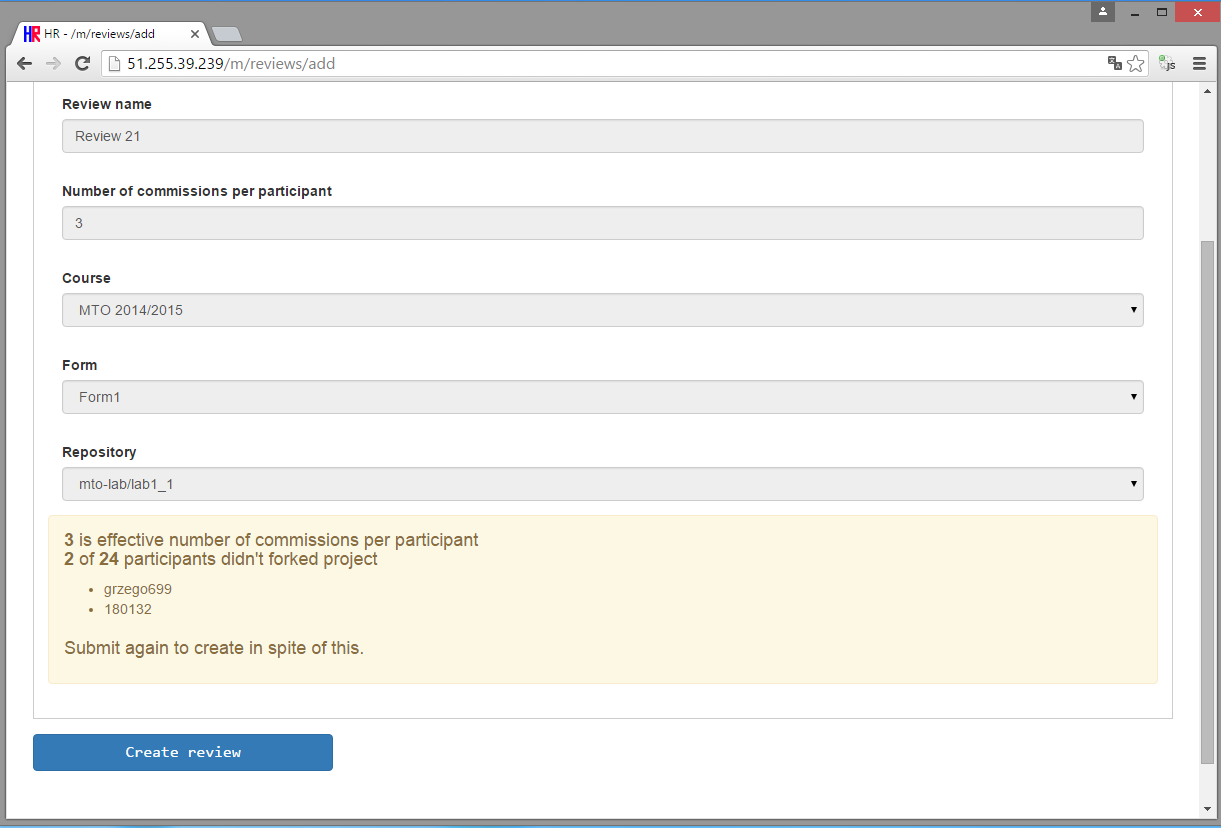
\includegraphics[width=405px]{5_2_3_radd2}
    \caption{Zrzut ekranowy: formularz dodawania przeglądu}
    \label{obr523}
\end{figure}

\clearpage
Rysunki numer \ref{kodp1} oraz \ref{kodp2} zawierają listing kodu źródłowego. Są to dwie części kodu z~klasy \textquote{GHReviewCreator}, która odpowiada za proces przygotowania przeglądu i~zarejestrowania wszystkich zleceń do wykonania. Pierwszy z~nich zawiera fragment do momentu sprawdzenia, ile osób nie wywiązało się z~zadania i~wyświetlenia tej informacji prowadzącemu, celem uzyskania potwierdzenia chęci kontynuacji. Po potwierdzeniu zastosowanie znajduje kod zamieszczony na drugim listingu. Funkcję, której listing zamieszczono wywołuje kontroler, odpowiedzialny za podstronę zlecania przeglądów. Przekazywany do niej zostaje wypełniony formularz (obiekt typu \textquote{GHReviewAddForm}), repozytorium z~zadaniem (obiekt typu \textquote{GHRepository)} oraz obiekt umożliwiający zmianę stanu wysyłanej odpowiedzi HTTP (\textquote{HttpServletResponse}). Funkcja zwraca numer nowo utworzonego przeglądu.

\begin{figure}[!h]
    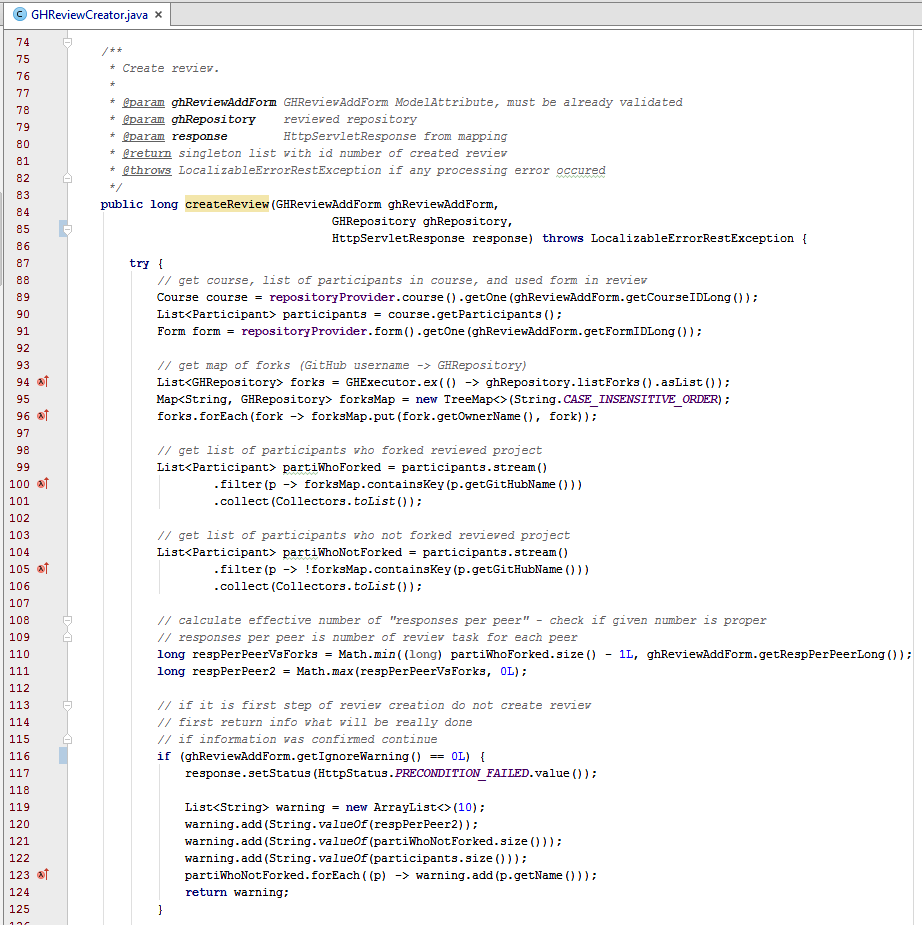
\includegraphics[width=\textwidth]{kod_przeglad}
    \caption{Listing kodu źródłowego: tworzenie przeglądu, klasa GHReviewCreator (część 1)}
    \label{kodp1}
\end{figure}

\begin{figure}[!h]
    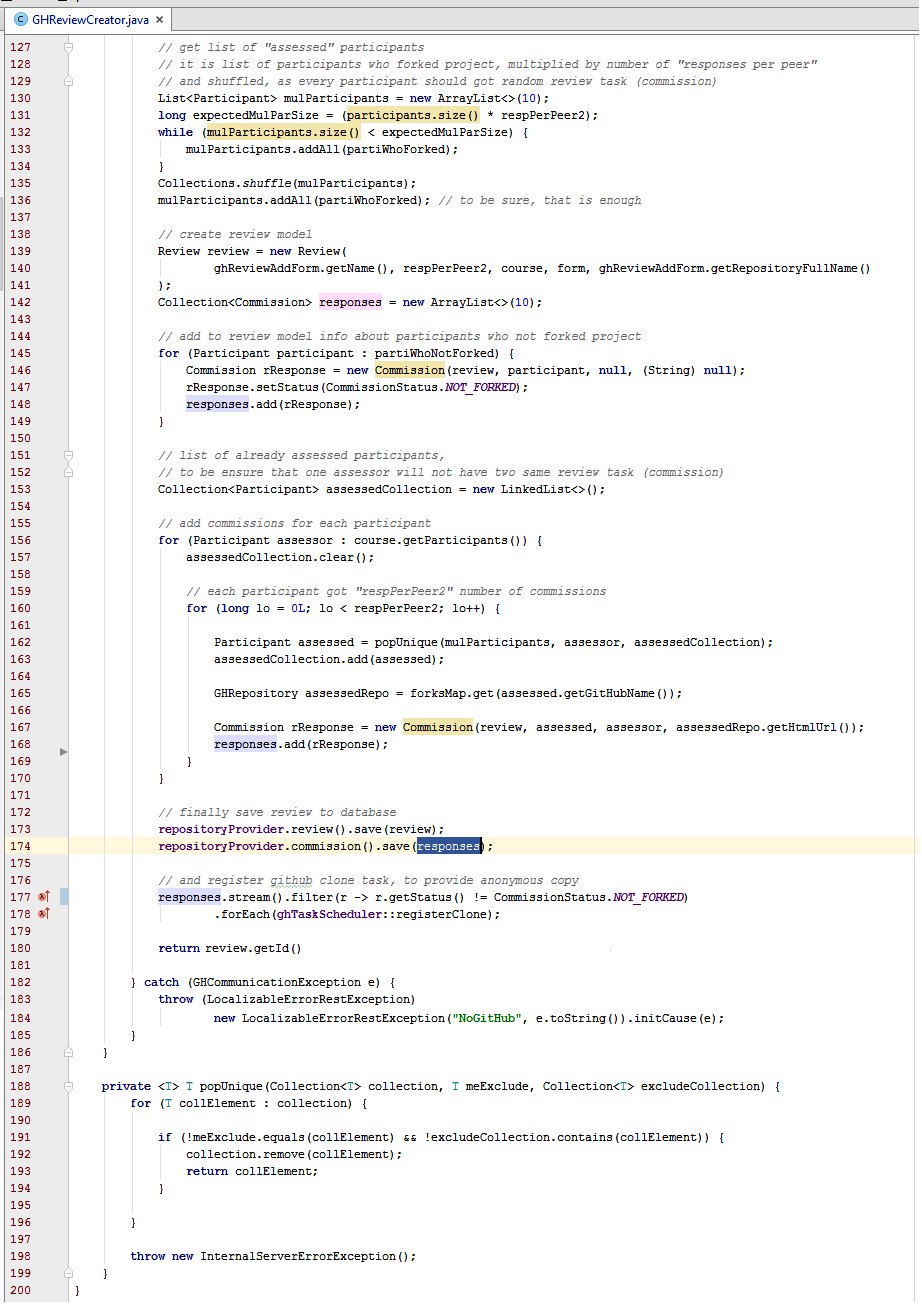
\includegraphics[width=\textwidth]{kod_przeglad2}
    \caption{Listing kodu źródłowego: tworzenie przeglądu, klasa GHReviewCreator (część 2)}
    \label{kodp2}
\end{figure}

\clearpage
\subsection{Algorytm anonimizacji prac}
Z momentem utworzenia przeglądu system uruchomił algorytm odpowiedzialny za anonimizację prac. W~tym momencie lista zleceń jest już znana, zostały ustalone adresy repozytoriów źródłowych - było to niezbędne już na wcześniejszym etapie. Dla każdego zlecenia system dokonuje kopiowania pracy. Za skopiowanie pracy jest odpowiedzialna klasa GHTaskClone. Proces kopiowania przebiega zgodnie ze schematem:

\begin{enumerate}
    \item system zgłasza zlecenie: Kursant1 ma ocenić pracę Kursant2;
    \item system nadaje zleceniu indywidualny unikalny ID, zgodny ze standardem UUID4;
    \item system zakłada repozytorium zdalne na koncie \textquote{manekin} (ang. dummy), którego token został podany w~pliku konfiguracyjnym, o~nazwie takiej, jak nadany ciąg ID;
    \item system sprawdza listę gałęzi (ang. branch) w~kopiowanym repozytorium;
    \item system kopiuje każdą ze znalezionych gałęzi:
    \begin{enumerate}
        \item system pobiera do folderu tymczasowego (zdefiniowanego znacznikiem \textquote{tempdir} w~pliku konfiguracyjnym) wybraną gałąź z~repozytorium źródłowego, na tym folderze wykonuje kolejne akcje;
        \item system usuwa ukryty folder \textquote{.git} - projekt przestaje być repozytorium Git;
        \item system inicjalizacje nowe puste repozytorium lokalne;
        \item system konfiguruje nowe repozytorium - nazwa użytkownika i~adres e-mail zostają ustawione na takie, które widnieją w~konfiguracji konta \textquote{dummy} na platformie GitHub;
        \item system zapisuje zmiany (w~tym przypadku: wszystkie istniejące pliki) w~repozytorium lokalnym (akcja git: commit), treścią używaną do opisu zmian jest ciąg \textquote{commitmsg} ustalony w~pliku konfiguracyjnym;
        \item system wysyła skopiowaną lokalnie gałąź do repozytorium zdalnego (git push);
    \end{enumerate}
    \item system sprawdza jaka gałąź w~repozytorium źródłowym jest ustawiona jako domyślna (ang. default), takiego samego ustawienia dokonuje na kopii;
    \item system zapisuje adres utworzonej kopii w~bazie danych - to ten adres zostanie przekazany recenzentowi.
\end{enumerate}

Jeżeli proces kopiowania nie powiedzie się, na jakimkolwiek etapie, zmiany są wycofywane. W~bazie danych zostaje zapisana odpowiednia informacja o~porażce. Niepowodzenie może być spowodowane wieloma czynnikami. Najprostszą przyczyną jest niedostępność jednej z~usług platformy GitHub. Inną możliwą przyczyną jest niedoskonałość implementacji algorytmu, który zawiódł z~bliżej nieokreślonej przyczyny - podczas testów przypadek taki został zanotowany dla około pół procent zleceń. Autor po konsultacji z~opiekunem pracy ustalił, że zbadana niezawodność jest wystarczająca. Proces ponowienia próby kopiowania nie jest dokonywany automatycznie, należy go uruchomić manualnie. System przewiduje odpowiednią opcję dostępną w~podglądzie stanów zleceń.

\medskip
\textquote{Esencję} algorytmu anonimizacji zawiera obrazek \ref{kodanon} na stronie \pageref{kodanon}. Jest to listing funkcji \textquote{run} z~klasy \textquote{GHTaskClone}. Wspominana klasa reprezentuje zadanie anonimizacji prac i~wykonuje kolejne czynności zgodnie z~zaprezentowanych schematem.

\medskip
Jak wspomniano, w~systemie istnieje możliwość podglądu stanów zleceń oceny w~ramach przeglądu. Podgląd ten został zaprezentowany na zrzucie ekranowym na obrazku numer \ref{obr524} na stronie \pageref{obr524}. Widniejący tam status może przyjąć następujące wartości:

\begin{itemize}
    \item projekt nie powielony (ang. project not forked) - informacja dodatkowa, wpis taki jest tworzony dla każdego kursanta, którego rozwiązanie nie zostało znalezione. W~sposób naturalny praca takiego kursanta nie może zostać oceniona. Sam kursant jednak oczywiście dostaje do oceny inne prace;
    \item przetwarzanie zakończone porażką (ang. processing failed) - proces kopiowania zakończył się niepowodzeniem. W~przypadku niepowodzenia obok zlecenia staje się dostępny przycisk pozwalający ponowić próbę (ang. retry) anonimizacji dla tej pracy;
    \item w~trakcie przetwarzania (ang. processing) - anonimizacja dla tego zlecenia została zaplanowana, lub jest w~trakcie przetwarzania. System kolejkuje zlecenia, wykonując jednocześnie nie więcej niż trzy kopie.
    \item ocena nie wypełniona (ang. unfilled) - proces anonimizacji zakończył się powodzeniem i~formularz oceny jest dostępny dla kursanta. Kursant nie dokonał jeszcze oceny;
    \item ocena wypełniona (ang. filled) - kursant dokonał oceny.
\end{itemize}

\medskip
Jak już zostało wyjaśnione kopie są składowane na specjalnie do tego przeznaczonym koncie. Obrazek \ref{526schemat} przedstawia schematycznie obieg repozytorium. Zrzut ekranowy na obrazku \ref{obr525} na stronie \pageref{obr525} przedstawia natomiast przykładową listę repozytoriów widoczną na takim koncie.

\begin{figure}[!h]
    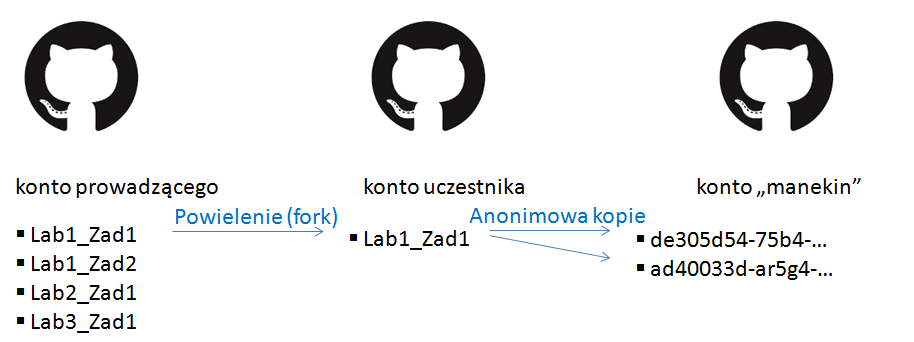
\includegraphics[width=290px]{5_2_6schemat}
    \caption{Repozytorium z zadaniem i jego powielenia nad kontach w usłudze GitHub}
    \label{526schemat}
\end{figure}

\begin{figure}[!h]
    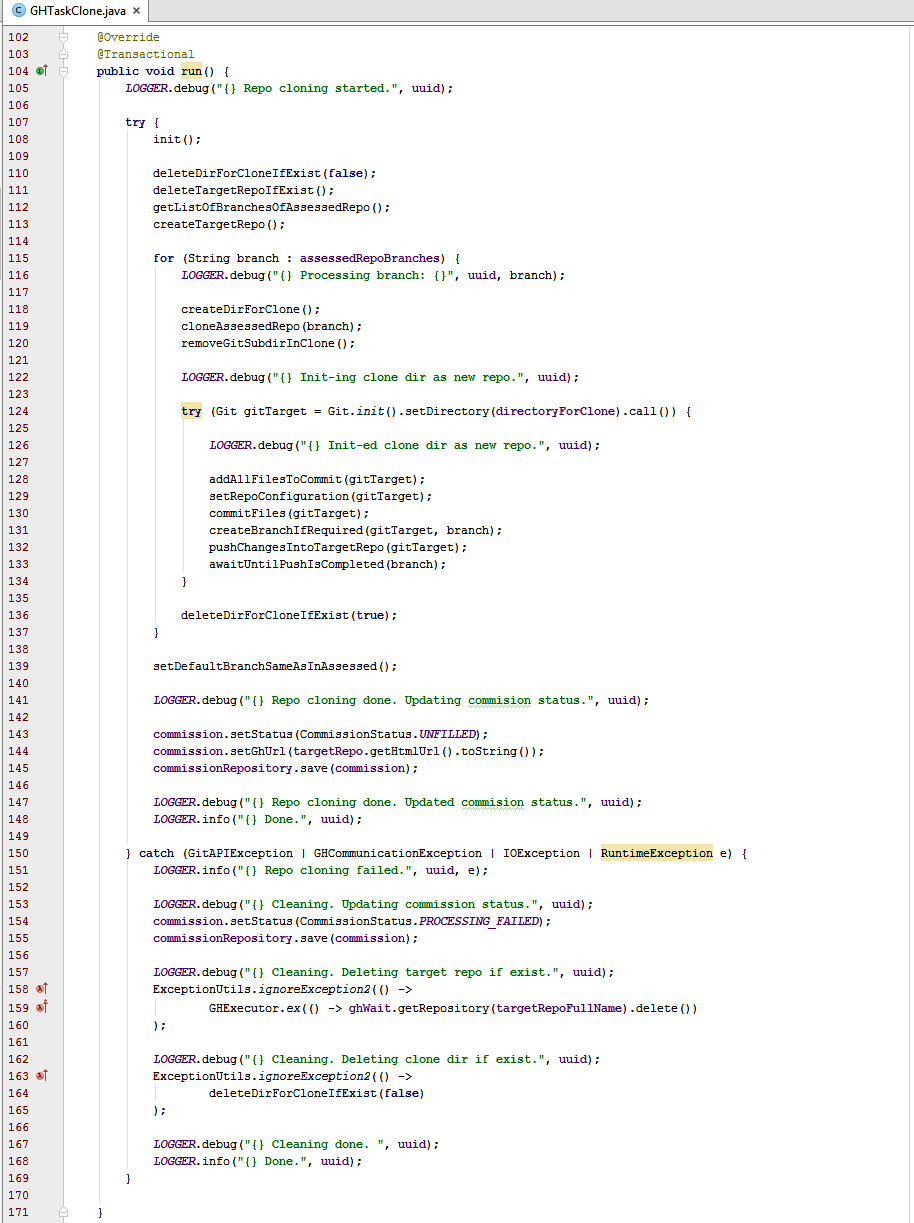
\includegraphics[width=\textwidth]{kod_klonowanie}
    \caption{Listing kodu źródłowego: anonimizacja prac, kopiowanie repozytorium}
    \label{kodanon}
\end{figure}


\begin{figure}[!h]
    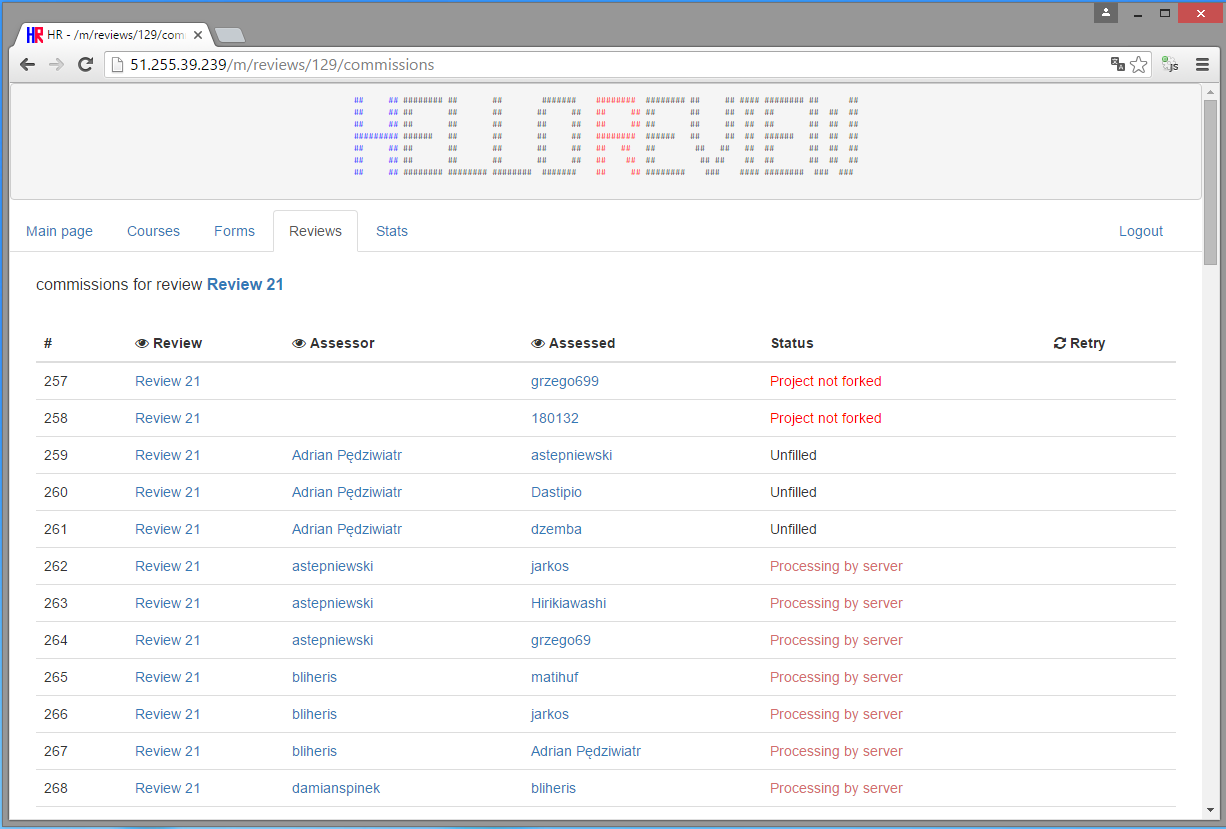
\includegraphics[width=\textwidth]{5_2_4status}
    \caption{Zrzut ekranowy: status zleceń w~przeglądzie}
    \label{obr524}
\end{figure}

\begin{figure}[!h]
    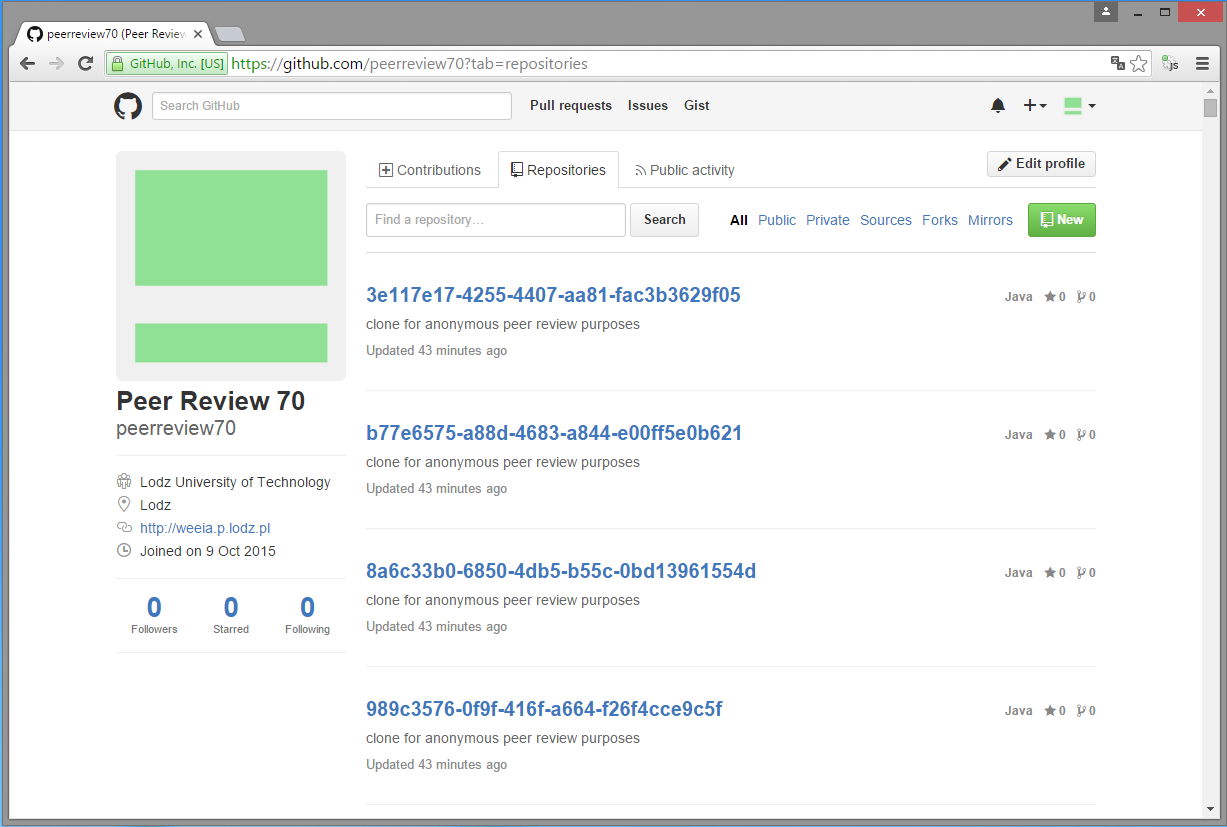
\includegraphics[width=\textwidth]{5_2_5dummyrepo}
    \caption{Zrzut ekranowy: anonimowe kopie zleceń w~usłudze GitHub}
    \label{obr525}
\end{figure}

\clearpage
\section{Kursant dokonuje oceny}
Kursant po zalogowaniu do systemu widzi listę zleceń. Rysunek ze zrzutem ekranowym numer \ref{obr61} przedstawia przykładową listę. Jeżeli zlecenie zostało już poprawnie przetworzone przez algorytm anonimizujący, przegląd nie jest zamknięty a~odpowiedź jeszcze nie udzielona użytkownik może wykonać przydzielone mu zadanie - dokonać przeglądu i~oceny pracy. Zlecenia takie zostały wyróżnione na liście szarym kolorem, oraz czerwoną lewą i~prawą krawędzią tabeli. Adres do formularza oceny znajduje się jako ostatnia pozycja na liście. Adres do formularza, sam formularz, ani żadna inna informacja nie ujawnia autora ocenianego rozwiązania. Kursant zna tylko indywidualny numer zlecenia, który nie zdradza tej informacji, ani nie daje się z niczym powiązać (między innymi z uwagi na zastosowaną losowość ID).

\begin{figure}[!h]
    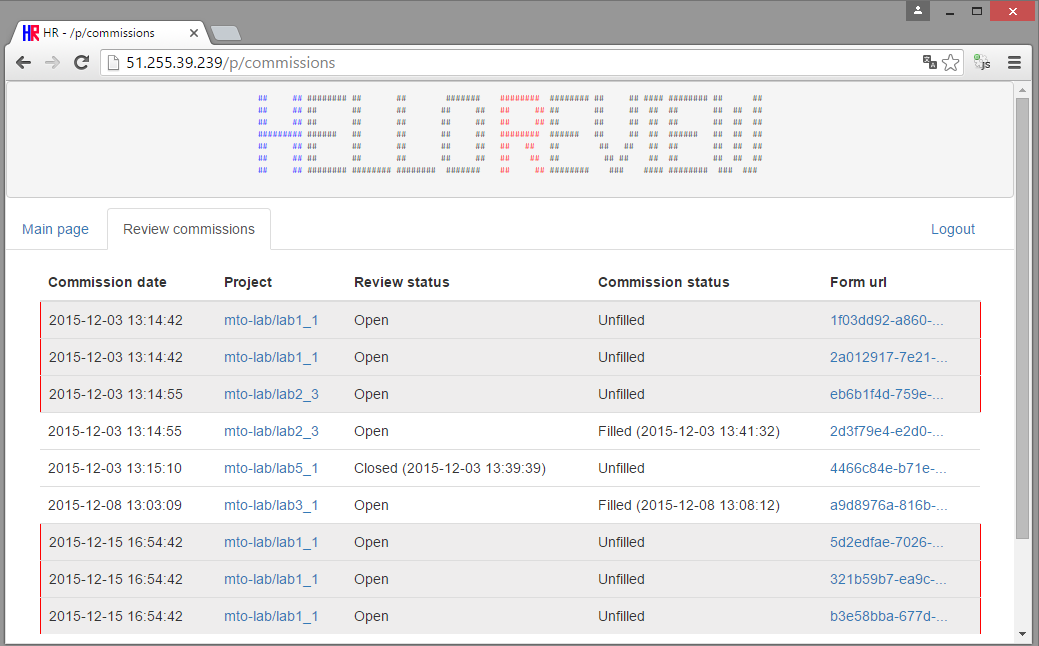
\includegraphics[width=\textwidth]{6_1zlecenia}
    \caption{Zrzut ekranowy: lista zleceń na koncie kursanta}
    \label{obr61}
\end{figure}

\medskip
Formularz wyświetlony użytkownikowi, jest identyczny z~tym, który prowadzący widział na podglądzie. Obowiązkowe kontrolki zostały oznaczone znakiem gwiazdki. Zrzut ekranowy na rysunku numer \ref{obr512} na stronie \pageref{obr512} przedstawia przykładowy formularz. Wyświetlenie formularza, na który już dokonano odpowiedzi skutkuje wyświetleniem formularza, na którym wszystkie kontrolki są w~trybie tylko do odczytu - użytkownik może się zapoznać z~dokonanymi odpowiedziami, ale nie ma już możliwości ich modyfikacji. Próba wyświetlenia formularza, związanego z~jeszcze nie przetworzonym zleceniem powoduje wyświetlenie komunikatu ze stosowną informacją - \textquote{Sorry, this form is not ready yet, it is not fully processed by server. Please wait 30 minutes, then contact the course master}.

\medskip
Kursant ma czas na dokonanie do czasu zamknięcia przeglądu. Zgodnie z~zastosowanym założeniem, po jego zamknięciu może on wyświetlić dokonane odpowiedzi, ale adresy do anonimowych kopii mogą być już nieaktywne, gdyż jako niepotrzebne mogły zostać już usunięte.

\section{Prowadzący sprawdza odpowiedzi}
Prowadzący posiada dwa źródła informacji o~stanie odpowiedzi. Pierwszym jest status zleceń, przedstawiony już na rysunku \ref{obr524} na stronie \pageref{obr524}. W~tym miejscu jest jednak tylko ogólna informacja kto dokonał oceny, a~kto jeszcze nie.

\medskip
Ponad to lista przeglądów (rysunek nr \ref{obr521} na stronie \pageref{obr521}) podsumowuje tą informację liczbowo. Wspominana informacja liczbowa jest odnośnikiem do szczegółów odpowiedzi. Nie ma możliwości podejrzenia ich poprzez podstronę systemu. Odnośnik ten prowadzi do generowanego dynamicznie arkusza Microsoft Excel gdzie znajdują się: stempel czasowy wygenerowania przeglądu, podsumowanie przeglądu, oraz wszystkie udzielone odpowiedzi. Prezentacja odpowiedzi w~arkuszu Excel pozwala w~łatwy sposób je filtrować i~przetwarzać. Przykład wygenerowanego arkusza zawiera rysunek nr \ref{obr71}.

\medskip
Prowadzący jest jedyną osobą, która zna odpowiedzi. W~jego gestii leży sposób ich wykorzystania. Może je uwzględnić wystawiając ocenę, przekazać grupie ogólne podsumowanie, każdemu z~osobna osobną informacje lub w~wykorzystać w~jakikolwiek inny sposób, który uzna za słuszny.

\begin{figure}[!h]
    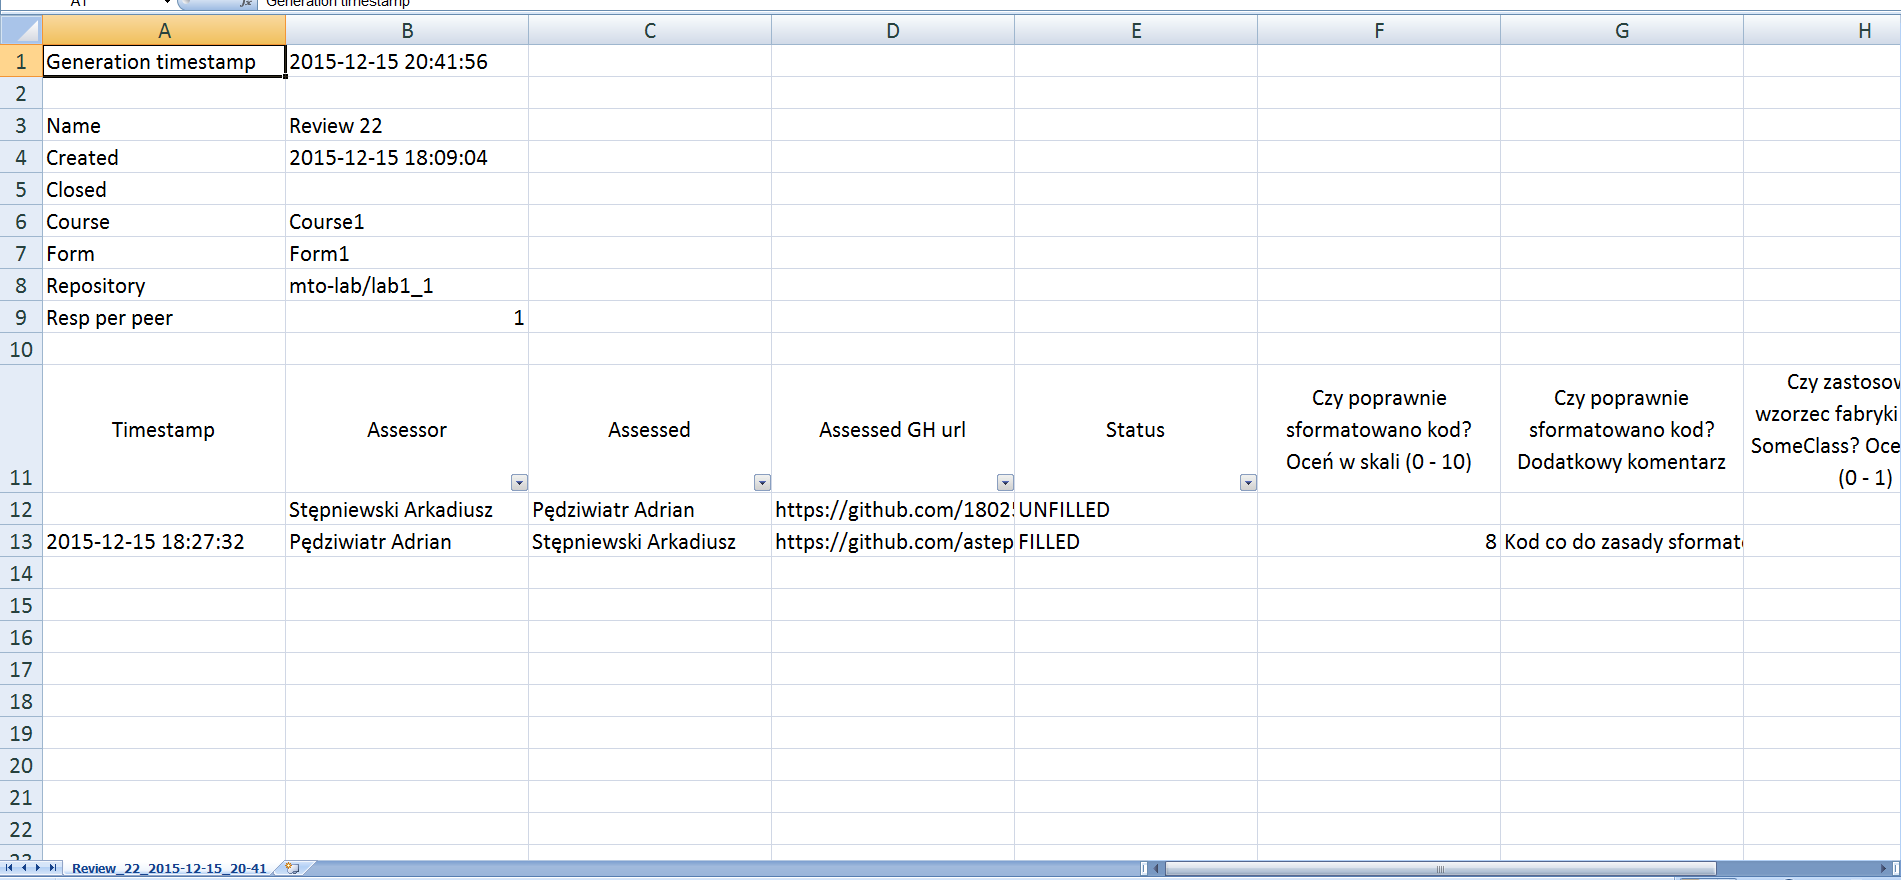
\includegraphics[width=\textwidth]{7_1excel}
    \caption{Zrzut ekranowy: arkusz MS Excel z~podsumowaniem dokonanych ocen}
    \label{obr71}
\end{figure}


\clearpage
\section{Statystyki systemu i~sprzątanie}
System posiada jeszcze jedną podstronę kontrolno-sprzątającą zaprezentowaną na rysunku \ref{obr81}. Znajdują się na niej informacje statystyczne i~techniczne (ściśle związane ze sposobem implementacji, mogą być pomocne przy rozwiązywaniu problemów). Wśród wypisywanych informacji są takie dane jak:
\begin{itemize}
    \item wykorzystanie aktualnego limitu połączeń z~GitHub API;
    \item stan pamięci podręcznej - czy jest ona włączona, oraz możliwość zmiany stanu;
    \item stan pamięci podręcznej - ilość wykorzystanego miejsca, oraz możliwość skasowania zapamiętanych informacji;
    \item procentowy wskaźnik udziału pamięci podręcznej przy wykonywaniu żądań http;
    \item przybliżona liczba zgłoszonych zadań związanych z~anonimizacją prac (dana techniczna);
    \item przybliżona liczba zadań, związanych z~anonimizacją prac, oczekują w~kolejce do wykonania (dana techniczna);
    \item liczba zleceń, które mają w~systemie status przetwarzanych;
    \item liczba repozytoriów (anonimowych kopii) na koncie \textquote{manekin} (dummy), które nie mają pokrycia w~bazie danych i~nie są potrzebne. Do tej liczby zaliczają się także kopie związane z~zamkniętymi przeglądami. W~tym miejscu istnieje możliwość usunięcia ich z~konta;
    \item liczba folderów w~katalogu tymczasowym (powinna być równa zero, jeżeli brak jest zadań w~kolejce) (dana techniczna).
\end{itemize}

\begin{figure}[!h]
    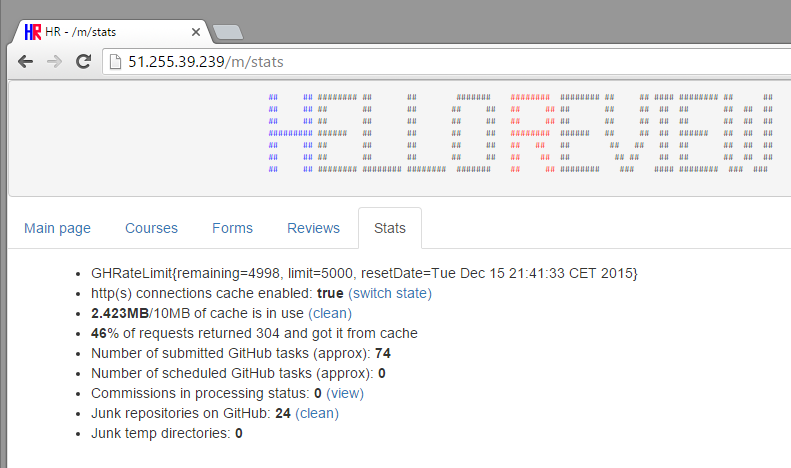
\includegraphics[width=400px]{8_1stats}
    \caption{Zrzut ekranowy: statystyki systemowe}
    \label{obr81}
\end{figure}


% ex: set tabstop=4 shiftwidth=4 softtabstop=4 noexpandtab fileformat=unix filetype=tex spelllang=pl,en spell:

